\chapter{Transformer} \label{ch:transformer}

This chapter introduces the development of ``transformer'' in its main branch. Transformer is an AI framework initially proposed in 2017 in a paper ``Attention is All You Need'', and it has magically revolutionized how we train AI for natural language processing and interpreting.

\section{It Seems That Attention is All You Need}

It started in 2017 when ``transformer'' is proposed in a paper ``Attention is all you need'', by Vaswani, et al., a bunch of guys mainly from Google.

``Attention'' was not a new concept previous to this paper. It was proposed a few years earlier than the transformer, and had been integrated into several CNN and RNN models to boost their performances to capture long-range dependencies. In these researches, attention mechanism is more often a supporting role than the main character. It is quite surprising indeed, that when getting rid of CNN and RNN and purely relying on attention mechanism, everything actually gets better: it is faster to train the network, and its performance gets improved.

Does this mean the RNN, which we had been relying on so much, is in fact the drawback to natural language processing? The following is the answer of ChatGPT-4 of this question.

\begin{shortbox}
	\textbf{Q: By getting rid of RNN and using attention mechanism alone, natural language processing performance gets better. Is this correct? Does this mean that RNN is a drawback to natural language processing?}
	
	A: Yes, by getting rid of RNNs and using the attention mechanism alone, the Transformer model demonstrated improved performance in natural language processing tasks. However, it's important to note that RNNs are not inherently a drawback to NLP; they were successfully used for many tasks before the advent of Transformers.
	
	RNNs, particularly LSTM (Long Short-Term Memory) and GRU (Gated Recurrent Unit) variants, were designed to handle sequences and capture dependencies in the data. They have been effective in many NLP tasks, such as language modeling, machine translation, and sentiment analysis. However, RNNs do have certain limitations, such as difficulty in capturing long-range dependencies and sequential processing, which can lead to slower training and inference times.
	
	The attention mechanism, as employed in the Transformer model, addresses some of these limitations. It enables parallel processing of input sequences, leading to faster training and inference, and effectively captures long-range dependencies without the vanishing gradient problem that can affect RNNs.
	
	While Transformers have shown superior performance in many NLP tasks, RNNs still have their place in certain scenarios, especially when working with resource-constrained environments or smaller datasets. They can be more lightweight and computationally efficient compared to large-scale Transformer models.
	
	In summary, RNNs are not a drawback to NLP per se, but their limitations have been mitigated by the introduction of the attention mechanism in Transformer models, which has led to improved performance in a wide range of NLP tasks.
	
	(April 14, 2023, ChatGPT-4)
\end{shortbox}

In the remaining part of the chapter, a quick review of CNN and RNN is given and their limitations introduced. Attention mechanism is illustrated. The original transformer model is explained. Finally, research trends of transformer as of today are briefly summarized.

\section{CNN, RNN, and Their Limitations}

This section does not focus on the detailed introduction of CNN and RNN mechanisms. Instead, only their main features are reviewed, and their limitations discussed. This section does not reflect on the state-of-art of researches in CNN and RNN.

The conventional feedforward network (network without cycles) with dense ANN is widely used. It can be trained systematically using back-propagation methods such as stochastic gradient descent. However, dense ANN is not very good at interpreting correlations among the inputs. At least, it is not good at doing it efficiently.

For example, consider the input to be pixels of an image of size $3\times 128 \times 128$, where $3$ corresponds to the RGB of the image, and $128 \times 128$ its pixel size. It is obvious to a human that the pixel at $(1,1)$ should definitely has a closer relationship with the one at $(1,2)$ (they are probably forming an object in the image together) than $(128, 128)$. The same applies to sequential inputs. Consider a signal sampled continuously. The first and second samples are very likely to be more strongly correlated than the first and last samples.

In a conventional dense ANN, the correlation cannot be captured efficiently. In contrast, a dense ANN would treat all the inputs ``equally'' in a symmetric manner. To enforce the ANN to ``memorize'' the correlation, it would require a lot more layers and nodes (which is often considered low-efficient), and requires more data points during the training. Other problems of conventional dense ANN include, for example, the lack of ability in handling data with arbitrary length.

CNN and RNN try to tackle the above problems by implementing a ``pre-processing'' stage, where the correlation of the spacial and sequential data is first abstracted using some mechanism, and the correlation information is sent as (additional) inputs to the followed dense ANN.

The details of CNN and RNN mechanisms are not discussed in this notebook. Brief reviews are given as follows.

\subsection{Brief Review of CNN}

CNN is a type of ANN structure designed to handle grid-like data. It is effective when dealing when data spatially correlated, thus becomes very popular in computer vision. It defines ``kernel'' that aggregates nearby pixels information before sending it to a dense network.

A CNN kernel, also known as a filter, is a small matrix of weights that slides across the input image or feature map to perform a mathematical operation called convolution. An demonstration of CNN kernel is given in Fig. \ref{ch:transformerbasics:fig:cnn_kernel}. Multiple kernels can be defined on the same layer to handle the same feature map, each kernel associated with an output channel. In practice, each kernel or channel is designed to detect a specific features in the feature map. For example, there might be a kernel detecting edges, while a second kernel detect color codes.

\begin{figure}
	\centering
	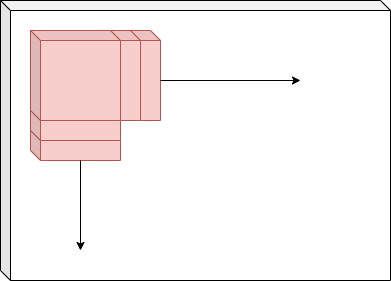
\includegraphics[width=200pt]{chapters/ch-transformer/figs/cnn_kernel.png}
	\caption{A demonstration of CNN kernel. The input is given by the white box (3D), and the kernel by the red box.} \label{ch:transformerbasics:fig:cnn_kernel}
\end{figure}

Notice that CNN differs quite largely from transformer in the problems they are expected to address. CNN is more for spatial data processing such as image processing, while transformer targets more on sequential data processing such as natural language processing and machine translation.

\subsection{Brief Review of RNN}

RNN is a connectionist model with the ability to selectively pass information across sequence steps \cite{lipton2015critical}. It is good at handling sequence of data such as voice message, text contents, or a flow of images (videos). It is worth mentioning that the ``sequence'' does not necessarily mean a time sequence. Nevertheless, without losing generality, we will consider time sequence in the review for simplicity and convenience.

Denote inputs $x(1), x(2), ..., x(k), ...$ where $x(k)$ is a vector sampled at time instant $k$. The length of the sequence may be finite or infinite. In the case of finite sequence, its maximum sample index is denoted by $T$. For example, in the context of natural language processing, each input might be a word in a dictionary. For example, $x(1) = \textup{``Pandas''}$, $x(2)=\textup{``are''}$, $x(3)=\textup{``so''}$, $x(4)=\textup{``cute''}$, $x(5)=\textup{``!''}$. The corresponding target output sequence is given by $y(1), y(2), ..., y(k), ...$, respectively.

RNN differs from the conventional dense ANN by introducing ``recurrent edges'', which allows the output of hidden layers at $k-1$ be used as additional inputs to the system at $k$. This means, at any time $k$, the input of the system includes both $x(k)$ and also selected $h(k-1)$, where $h(\cdot)$ is the outputs of hidden layers. We can think of the ``weights'' of a trained RNN the ``long-term memory'' that does not change with specific sequence of inputs, while the information passing through recurrent edges the ``short-term memory'' that links previous inputs with future inputs.

A demonstration is given in Fig. \ref{ch:transformerbasics:fig:rnn_general}. Notice that each hidden layer is a multi-input-multi-output subsystem containing multiple nodes. Different from a conventional dense ANN, each hidden layer takes additional inputs from its corresponding hidden layer in the previous instant. It is also common to see ``bypass'' (this is widely used in different ANN structures, not unique to RNN) for better performance of the system.

\begin{figure}
	\centering
	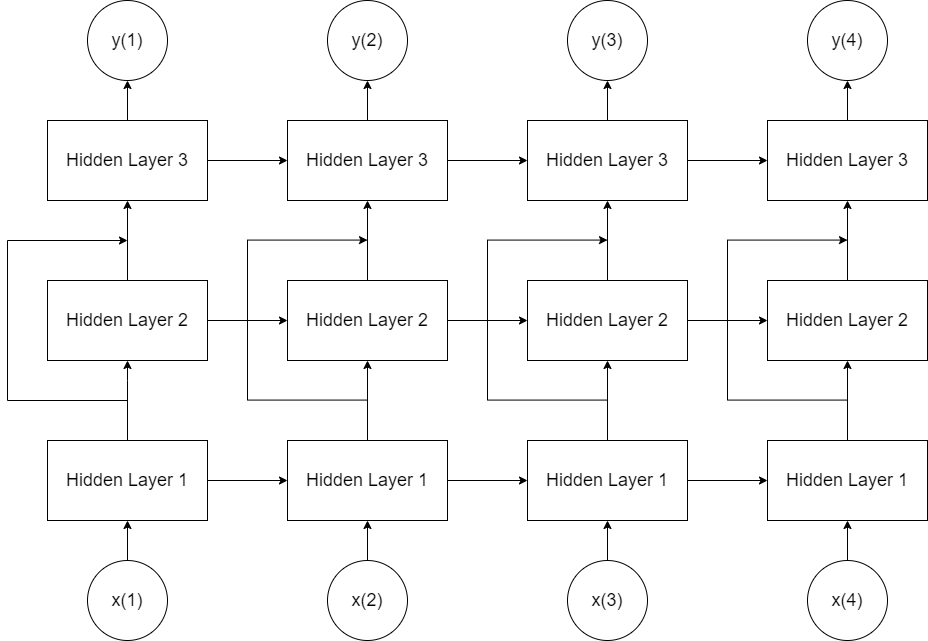
\includegraphics[width=250pt]{chapters/ch-transformer/figs/rnn_general.png}
	\caption{A example of RNN.} \label{ch:transformerbasics:fig:rnn_general}
\end{figure}

RNN has some limitations. One of the major problem is that it is difficult to train an RNN even for the basic standard feedforward networks. The optimization of RNN is NP-complete. It is especially difficult for RNN to learn long-range dependencies due to the vanishing and exploding gradients problem that could occur when backpropagating errors across many timestamps (long sequence) \cite{lipton2015critical}. This is one of the main challenges why RNN has difficulties building on long-range dependencies. The vanishing and exploding gradient problems are caused by the structure of the system as well as the backpropagation-based training methods.

Different approaches have been proposed to prevent vanishing and exploding gradient problems. Famous ones among these approaches include strategical weight initialization, long short term memory (LSTM), gated recurrent units (GRUs), skip connections, and more. Many of these approaches try to reduce the effect of vanishing and exploding gradient problems by carefully design the ANN structures. For example, both LSTM and GRUs introduce ``memory cells'' with built-in ``gates'' that balance and control the flow of information from previous cells versus current inputs. The cells are used to replace the traditional perceptron nodes. These approaches have made the training of RNN a feasible problem. LSTM and GRUs are almost certainly used in modern RNNs.

Bidirectional RNN (BRNN) is proposed at about the same time with LSTM. It allows information to travel not only from previous hidden layers to future layers, but also from future hidden layers to previous layers. LSTM and BRNN can be used together to boost the RNN performance. Notice that BRNN cannot run continuously as it requires fixed endpoints in both the future and the past. It is useful for prediction over a sequence of fixed length, such as part-of-speech tagging in natural language processing.

Another problem that people have found during the training of RNN is local optima. However, recent studies have shown that local optima is not as serious issue as we might thought when the network is large, since many critical points are actually saddle points rather than local minima.

Successful implementations of the above RNN structures include natural language translation such as \cite{sutskever2014sequence} where a encoder-decoder structure is used, each is a LSTM. Another example is image captioning, where the AI tries to explain what is in an image using texts. A solution to this is to use CNN to encode the image, and use LSTM to decode to generate texts. Following similar ideas is hand-writing reorganization.

\section{Attention Mechanism}

\section{Transformer}

While CNN is mainly used for spatial data processing such as computer vision, both RNN and transformer are mainly used for sequential data processing. It is worth mention in the very beginning that transformer does not guarantee superior performance in all scenarios comparing with traditional RNN-based natural language processing models such as LSTM.

For one thing, transformer consumes larger computational capabilities. Transformer processes data in batch, while RNN does them in sequence, meaning that RNN can response faster in some real-time applications. It is difficult for the transformer to process super-long text due to the computational burden (quadratic computational complexity with respect to sequence length), while RNN can process arbitrarily long text, although the later suffers from capturing long-range dependencies.

With the above been said, the transformer does demonstrated superior performance than RNN in many tasks. The mechanism and the reasons why it performs better in these occasions are introduced as follows.

\section{Research Trends} 